\documentclass{standalone}
\usepackage[T1]{fontenc}
\usepackage[latin2]{inputenc}
\usepackage[english]{babel}
\usepackage{tikz}
\usetikzlibrary{calc,through,backgrounds,positioning,fit}
\usetikzlibrary{shapes,arrows,shadows}
 
\begin{document}
 
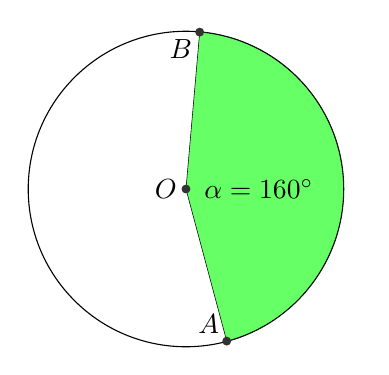
\begin{tikzpicture}[scale=1,inner sep=0.4mm]
\coordinate (O) at (0,0);
\coordinate (A) at (-75:2cm);
\coordinate (B) at (85:2cm);
\draw(0,0) circle(57pt);
\fill[green!60!white,very thin, draw=black]
(0,0) -- (-75:2cm)arc(-75:85:2) --cycle;

\node at (O) [circle,fill=black!80!white] {};
\node at (A) [circle,fill=black!80!white] {};
\node at (B) [circle,fill=black!80!white] {};

\node at (O) [left=2pt] {$O$};
\node at (O) [right=2pt] {$~\alpha = 160^\circ$};
\node at (A) [above left=2pt] {$A$};
\node at (B) [below left=2pt] {$B$};


\end{tikzpicture}
 
\end{document}